\documentclass[a4paper]{article}

%use the english line for english reports
%usepackage[english]{babel}
\usepackage[english]{babel}
\usepackage[utf8]{inputenc}
\usepackage{indentfirst}
\usepackage{graphicx}
\usepackage{verbatim}
\usepackage{url}
\usepackage{footnote}
\usepackage{eufrak}
\usepackage[hidelinks]{hyperref}
\usepackage{chngpage}

\begin{document}

\setlength{\textwidth}{16cm}
\setlength{\textheight}{22cm}

\title{\Huge\textbf{Order picking}\linebreak\linebreak\linebreak
\Large\textbf{Final report}\linebreak\linebreak

\includegraphics[height=6cm, width=7cm]{feup.pdf}\linebreak \linebreak
\Large{Master in informatics and computer engineering} \linebreak \linebreak
\Large{Information Systems}\linebreak
}

\author{\textbf{Group:}
\\ Duarte Nuno Pereira Duarte - 201109179 - ei11101@fe.up.pt
\\ Luís Filipe Correia Cleto - 201104279 -  ei11077@fe.up.pt
\\ Miguel Rui Pereira Marques - 201109178 - ei11099@fe.up.pt 
\\ Ruben Fernando Pinto Cordeiro - 201108177 - ei11097@fe.up.pt 
\\\linebreak\linebreak \\
 \\ Faculdade de Engenharia da Universidade do Porto \\ Rua Roberto Frias, s\/n, 4200-465 Porto, Portugal \linebreak\linebreak\linebreak
\linebreak\linebreak\vspace{1cm}}
\maketitle
\thispagestyle{empty}
\nocite{*}

%************************************************************************************************
%************************************************************************************************

\newpage

\tableofcontents

\newpage

%************************************************************************************************
%************************************************************************************************

%*************************************************************************************************
%************************************************************************************************

\section{Introduction}

The order picking or order preparation operation is one of a logistic warehouse's process. It consists in taking and collecting articles in a specified quantity before shipment to satisfy customers' orders. It is a basic warehousing process and has an important influence on the supply chain's productivity.

The putaway is an internal logistics process that comprises a set of tasks from receipt of a load to when it is stocked in its final destination within a warehouse.

The goal of the system as a whole is to optimize and automate this process step.

\newpage

\section{Added value}

The Management Information System will be used to support the decision of the order picker regarding the logistics of the order shipping and storage inside the warehouse. The client application will be used in a mobile setting.

The application will enable the order picker to:

\begin{itemize}
	\item See the pending orders from customers.
	\item Generate a picking list from customer orders, indicating the location of the items to be sent for shipping.
	\item See the pending orders from the suppliers.
	\item Generate a putaway list from pending orders from the suppliers.
\end{itemize}

\newpage

\section{Solution architecture}

The application architecture follows a client-server model, as shown in the following diagram:

\begin{figure}[h!]
\centerline{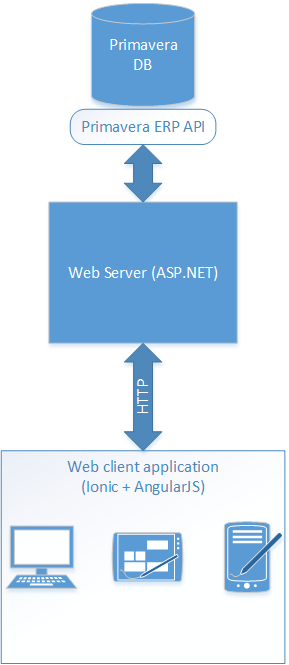
\includegraphics[height=8cm, width=3cm]{sinf_architecture_diagram.png}}
\caption{Application architecture diagram}
\end{figure}

The server was implemented with the ASP.NET framework, as explained in section~\ref{sec: aspnet}. The client was implemented with Ionic Framework and AngularJS, as explained in the sections~\ref{sec: ionic} and~\ref{sec: angular}.

\newpage

\section{Adopted Technologies and frameworks}

\subsection{ASP.NET}
\label{sec: aspnet}
ASP.NET is an open source server-side Web application framework. We did not use this framework to develop the website, instead, we used this framework in order to implement the REST API server. The language of choice was C\#.

Since the Primavera ERP API is also implemented with .net and C\#, no additional overhead was introduced server side.

\subsection{Ionic framework}
\label{sec: ionic}

Ionic is an open source HTML5 Mobile Framework for building cross-platform hybrid native apps with HTML, JavaScript, and CSS.

\begin{figure}[h!]
\centerline{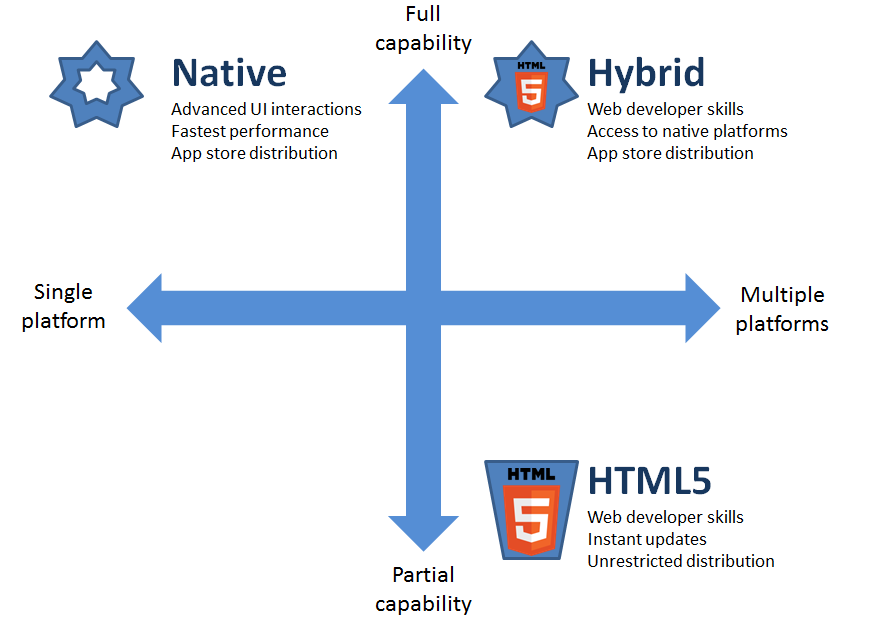
\includegraphics[height=8cm, width=13cm]{nativeVsHybrid.png}}
\caption{Native vs hybrid applications comparison diagram}
\end{figure}

This framework provides many UI components that work seamlessly across multiple mobile platforms, which are the target devices of this application. It also provides a hybrid deployment solution that combines:

\begin{itemize}
	\item Cross platform functionality provided by the web technologies.
    \item Platform affinity and performance provided by the web view engine bundled with Ionic: Cordova\footnote{\url{http://cordova.apache.org/}}.
\end{itemize}

\newpage

\subsection{AngularJS}
\label{sec: angular}

Instead of a set of static HTML pages, our client application is an AngularJS single page application. AngularJS is a javascript MVVM\footnote{Model-View-View-Model} framework.

\begin{figure}[h!]
\centerline{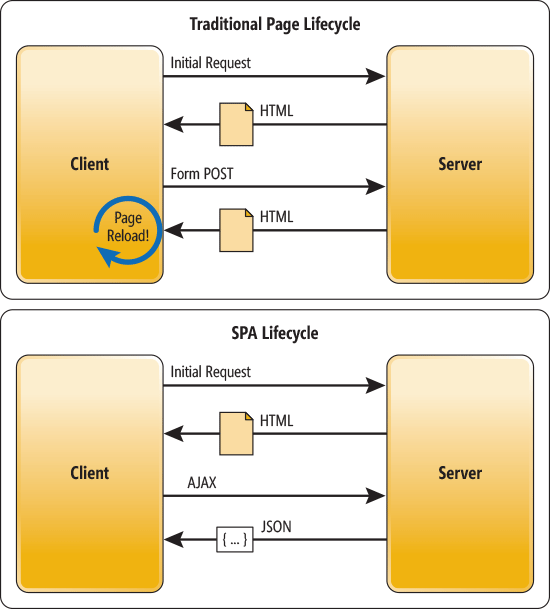
\includegraphics[height=6cm, width=7cm]{spa_diagram.png}}
\caption{Single Page Application diagram}
\end{figure}

The adoption of this framework had several design goals:

\begin{itemize}

	\item Decouple DOM manipulation from application logic. This substantially reduced boilerplate code and improved modularity and testability.
    
    \item Decouple the client side of the application from the server side. This reduced much of the burden on the backend and allowed development work to progress in parallel with minor hiccups.
    
    \item Provide an incremental and iterative development process for the client, from the UI design to the writing of the business logic.

\end{itemize}

\newpage

\section{User stories}

The following table contains the user stories for the application:
\begin{table}[h!]
\begin{adjustwidth}{-.7in}{-.7in}
\begin{tabular}{|l | l|}
\hline
User Story & Description \\ \hline
US-001 &
As a User I want to login in the application. \\ \hline
US-002 &
As a User I want to see the customer orders to be picked for shipping. \\ \hline
US-003 &
As a User I want to generate the picking list based on a set of orders from clients. \\ \hline
US-004 &
As a User I want to see the orders from the suppliers to be stored in the warehouse (putaway).
\\ \hline
US-005 &
As a User I want to generate a putaway list based on a set of incoming orders. \\ \hline
\end{tabular}
\caption{User stories}
\end{adjustwidth}
\end{table}

\newpage

\section{Core views}

\subsection{UI01 - Customer orders}

The user can see the undelivered orders in this view. 

\begin{figure}[h!]
\centerline{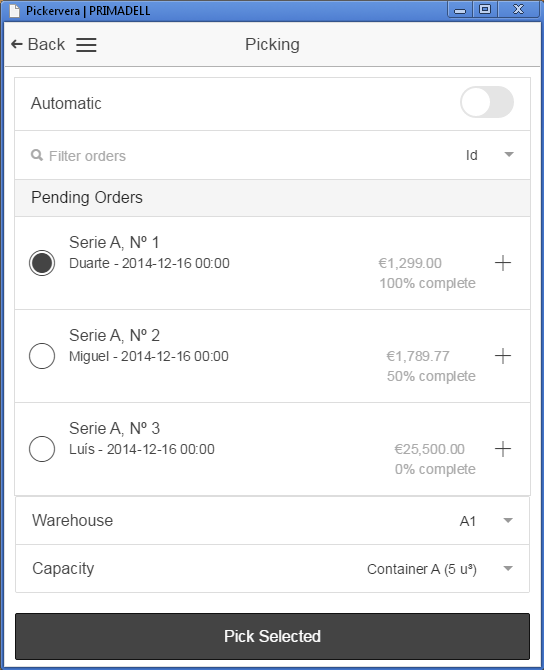
\includegraphics[width=9.5cm]{orders.png}}
\caption{Customer orders user interface}
\end{figure}

In order to generate a picking list for a set of orders from customers, he must choose the orders to process and press the "Pick Selected" button. After this, the user will be redirected to the Picking list view (see section~\ref{sec: picking}).

\newpage

\subsection{UI02 - Supplier orders}

The user can see the orders to be picked up from the suppliers in this view. 

\begin{figure}[h!]
\centerline{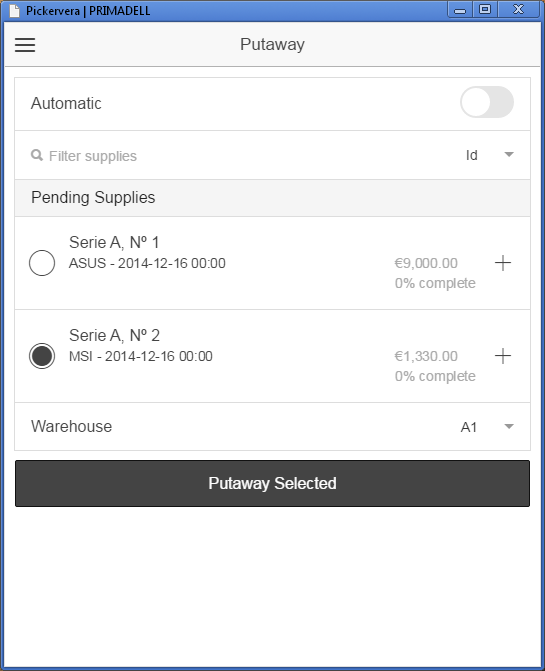
\includegraphics[width=9.5cm]{supplierOrders.png}}
\caption{Supplier orders user interface}
\end{figure}

In order to generate a putaway list for a set of orders, he must choose the orders to process and press the "generate putaway list" button. After this, the user will be redirected to the Putaway list view (see section~\ref{sec: putaway}). 
\newpage

\subsection{UI03 - Picking list}
\label{sec: picking}

In this view, the user can see the generated picking list for a set of customer orders. 

\begin{figure}[h!]
\centerline{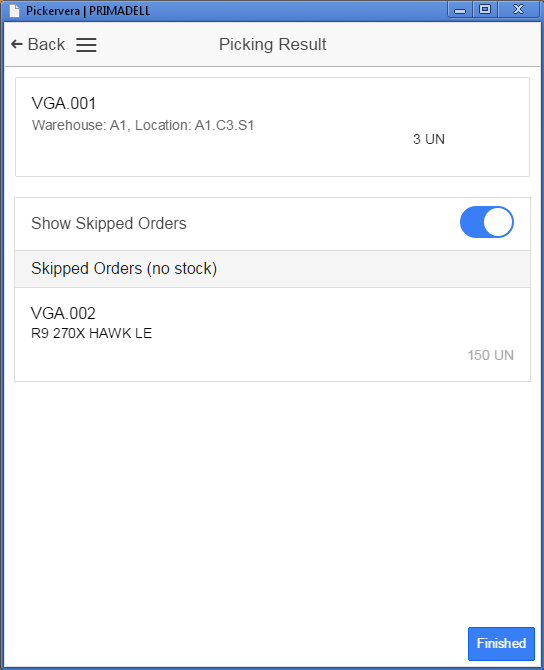
\includegraphics[width=9.5cm]{pickingList.png}}
\caption{Picking list user interface}
\end{figure}

Before the picking list is marked as finished, he must confirm the picked up quantities for each item in the list. Once all the picking item quantities are confirmed, the picking process is finished and the items are transfered from the warehouse to an output buffer.
\newpage

\subsection{UI04 - Putaway list}
\label{sec: putaway}

In this view, the user can see the generated putaway list for a set of supplier orders. 

\begin{figure}[h!]
\centerline{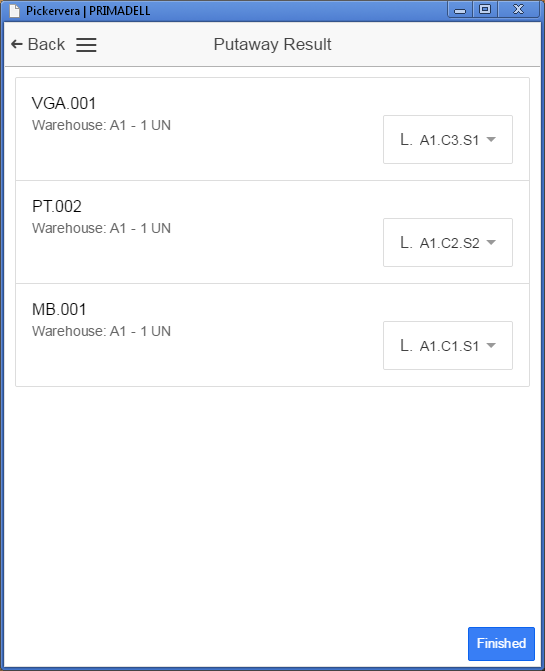
\includegraphics[width=9.5cm]{putawayList.png}}
\caption{Putaway list user interface}
\end{figure}

Before the putaway list is marked as finished, he must insert the location of the items in the warehouse. Once all the locations are confirmed, the putaway process is finished and the items are transfered into their respective locations.

\newpage

\section{The picking process}
\subsection{Algorithm}

The picking algorithm for a set of orders minimizes the distance that the picker has to travel while picking up and delivering the order items. It follows a greedy approach.

For a set of $\{O_1, O_2, ..., O_k\}$ orders, there is going to be a set of locations where the order items will be picked up. These locations, as their quantity, will be refered to as picking items.

Let $\{p_1, p_2, ..., p_w\}$ be the set of picking items to pick and $dist_{ij}$ be the distance for traveling from the location of $p_i$ to the location of $p_j$, the goal is to generate a sequence of picking items that minimizes the sum of the distances between the items, that is: 

\centerline{$\sum_{i,j}^{w} dist_{ij}$}

The order lines are first ordered by quantity. The algorithm then chooses the nearest location of the current picking item as the next place to travel to. 

This algorithm does not guarantee the best solution for the picking list generation, but it terminates in a reasonable amount of steps and provides a good solution in most cases.

\subsection{User interface scenario}
The batch picking process is rather simple with the application, as shown in the diagram below:

\begin{figure}[h!]
\centerline{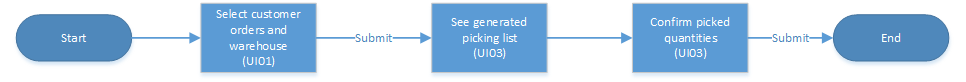
\includegraphics[height=1.6cm, width=16cm]{pickingDiagram.png}}
\caption{Generate picking list process}
\end{figure}

\subsection{Exceptional scenario}
There is a notable exception in the system in the picking process. When the amount of items to be picked in a location exceeds the available stock, a stock removal document is generated (\textit{"documento de saída de stock"}).

\newpage

\section{The putaway process}
\subsubsection{Algorithm}

The algorithm finds a suitable distribution of the order items by the warehouse while minimizing the traveling distance of the person responsible for the putaway.

The algorithm first tries to store the items in a location with the same items already stored. This is made so that there is minimal item dispersion in the warehouse.

If there are no locations with the same item already stored, the closest location is chosen. For two locations with the same distance, the one with the biggest amount of stock will be chosen.

The algorithm repeats this process for all the order items.

\subsubsection{User interface scenario}

The putaway process for the orders is very similar to the picking process. The process is shown in the diagram below:

\begin{figure}[h!]
\centerline{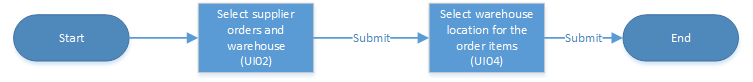
\includegraphics[height=1.8cm, width=16cm]{putawayDiagram.png}}
\caption{Generate putaway list process}
\end{figure}


\newpage

\section{Execution instructions and login information}
In order to initiate the system, execute the "Pickervera - PRIMADELL" file in the desktop, the server and the client will be started up automatically. If the browser does not open automatically, navigate to \textit{http://localhost/app}.

Login information:

\begin{itemize}
	\item Username: admin
	\item Password: admin
\end{itemize}

\newpage

\section{Notes}
\subsection{Warehouse configuration}
The warehouse locations were split into two dimensions: corridors and sections.

The numbering scheme of the locations is shown in the diagram below:

\begin{figure}[h!]
\centerline{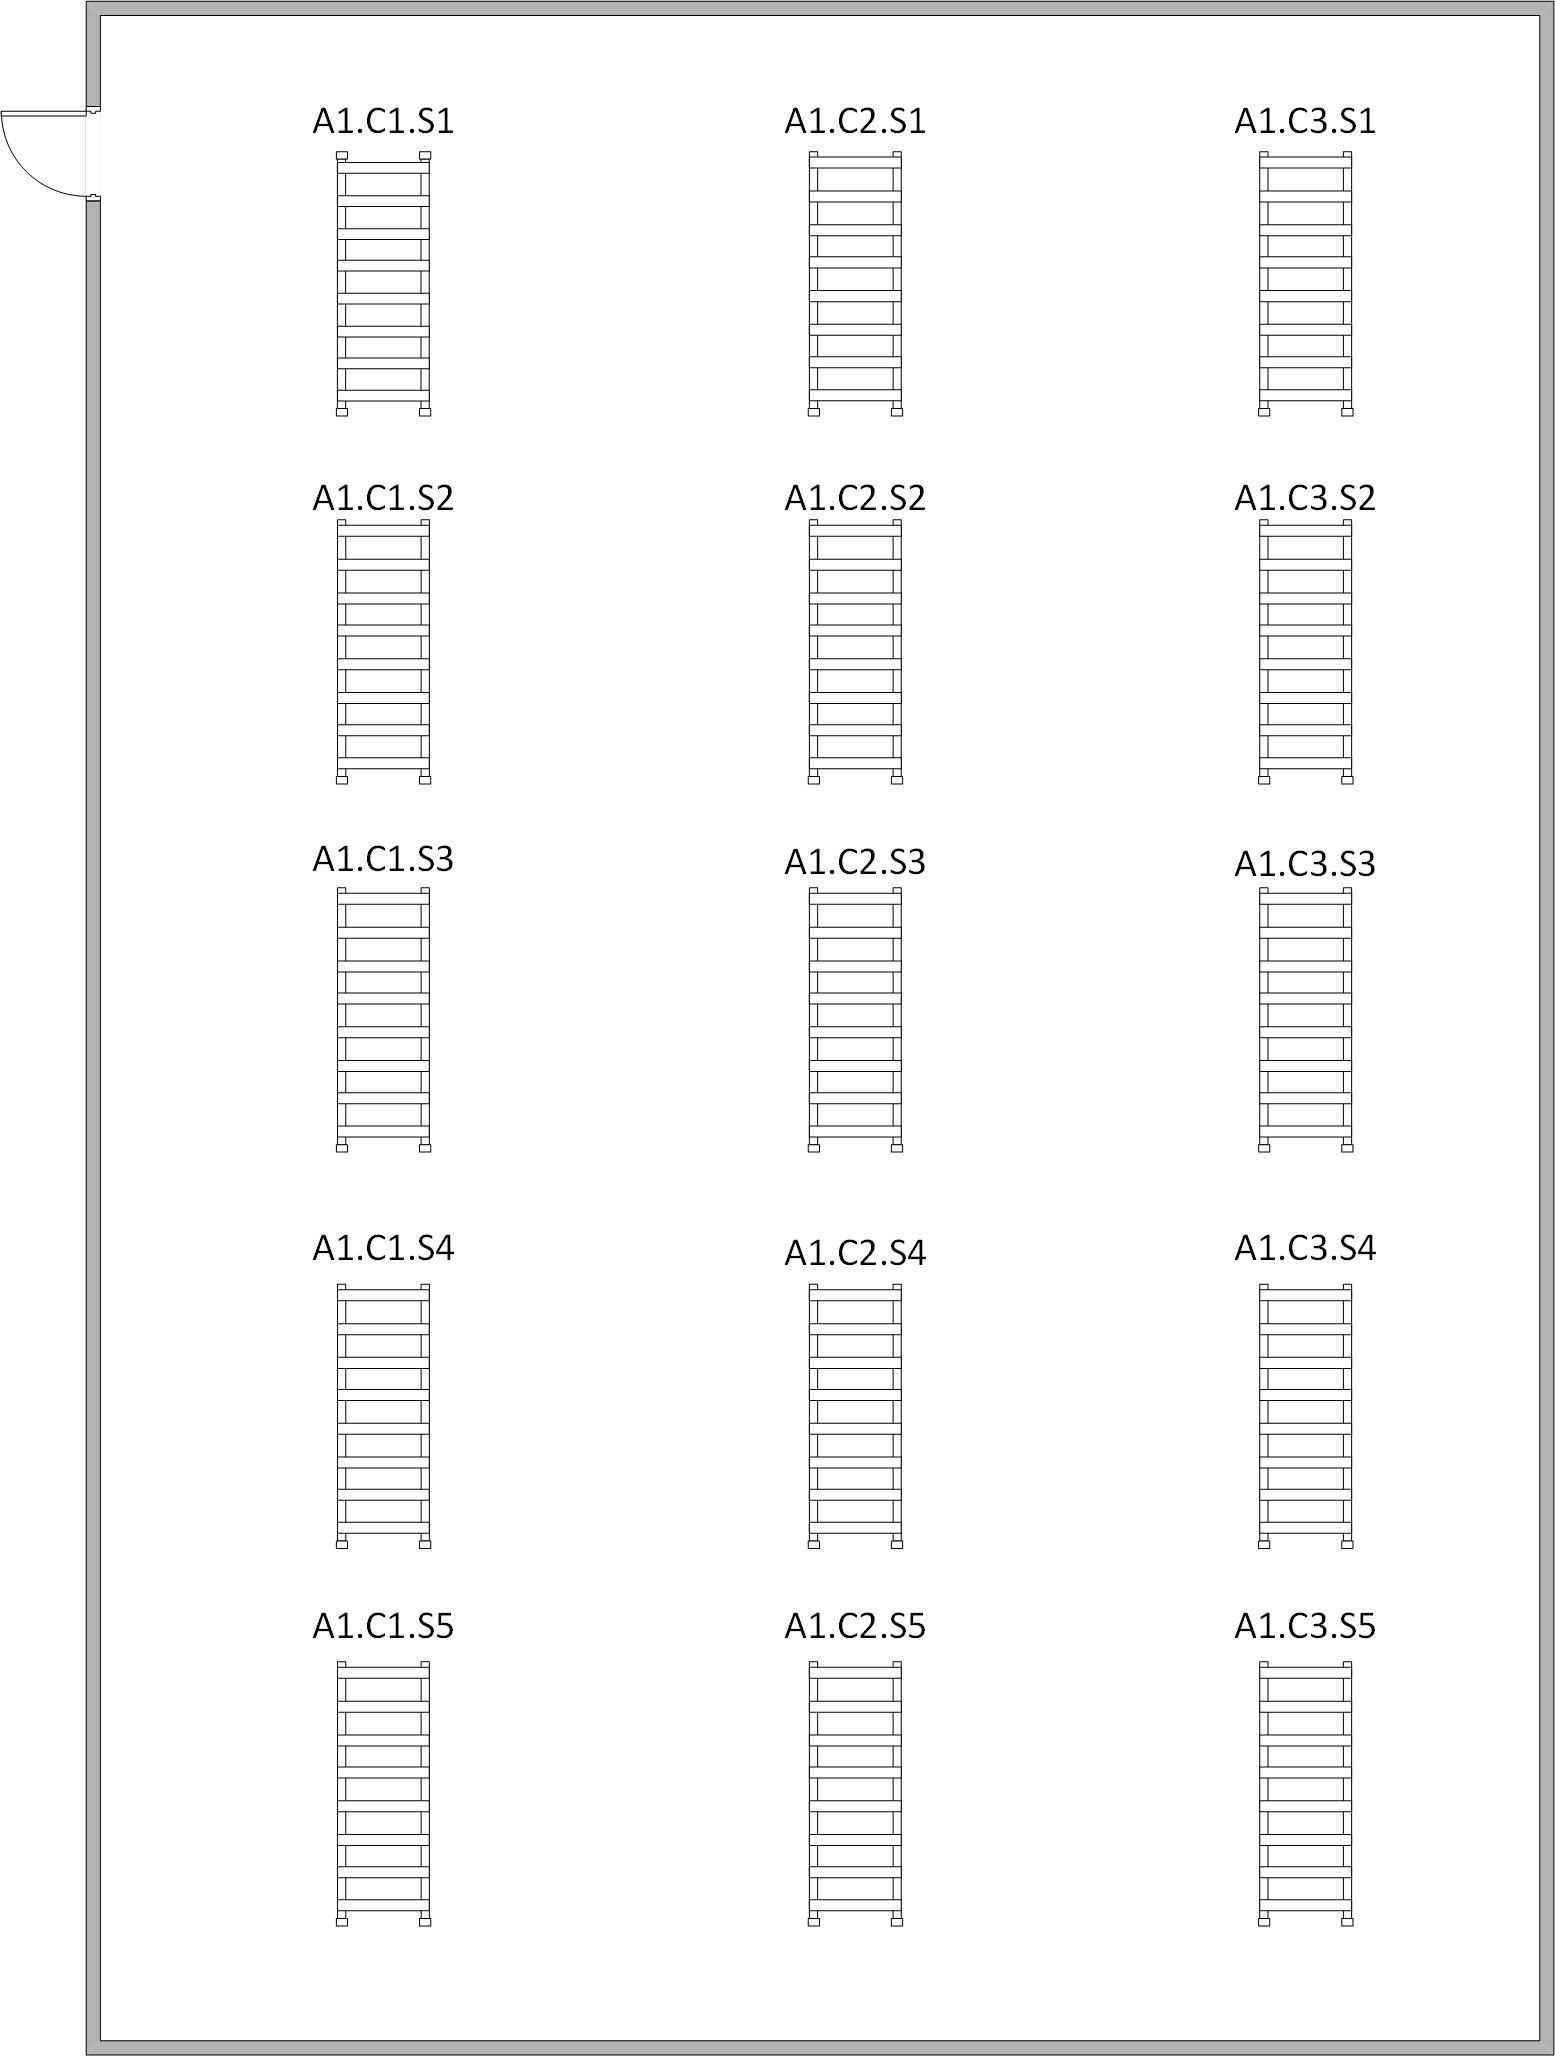
\includegraphics[height=14cm, width=12cm]{DrawingRacks.png}}
\caption{Warehouse location disposal diagram}
\end{figure}

\newpage

\subsection{Entity relationship diagram}
\begin{figure}[h!]
\centerline{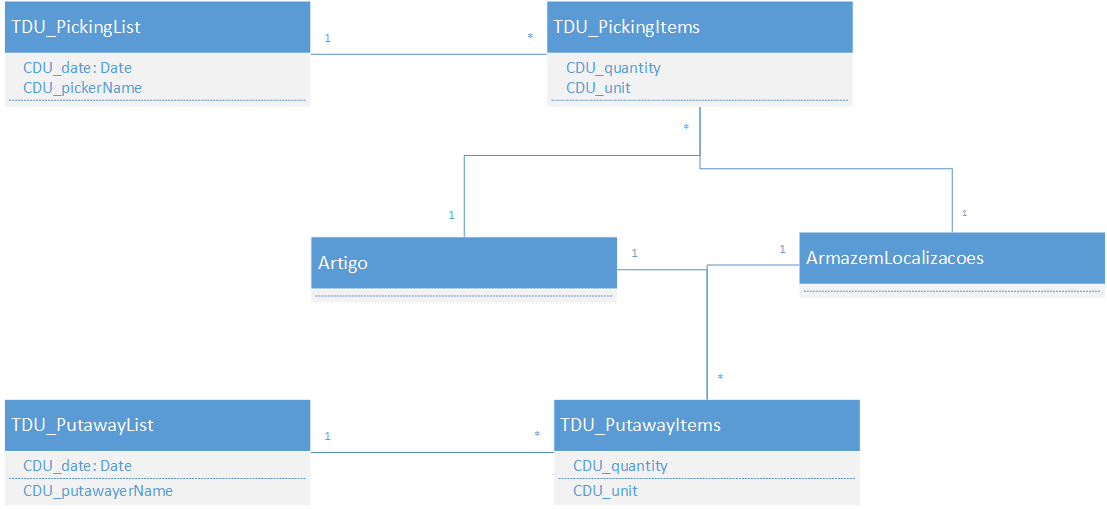
\includegraphics[height=8cm, width=16cm]{classDiagram.png}}
\caption{User tables entity relationship diagram}
\end{figure}

\newpage
\end{document}